\documentclass{iaf}

\annee{2017}

\usepackage[pdftex]{graphicx}
\usepackage{url}
\usepackage{amssymb,amsmath}
\usepackage{xspace}
\usepackage{tikz}
\usepackage[colorlinks,hyperindex,bookmarks,linkcolor=blue,citecolor=blue,urlcolor=blue]{hyperref}
\usepackage{mathrsfs} 
\usepackage{ifthen}

% Typo
\newcommand{\vs}{\emph{vs.}\@\xspace}
\newcommand{\touist}{\textsc{TouIST}\xspace}
\newcommand{\satoulouse}{\textsc{SAToulouse}\xspace}
\newcommand{\guill}[1]{\emph{#1}}
\newcommand{\etc}{\emph{etc.}\@\xspace}
\newcommand{\warning}[1]{\textcolor{red}{#1}}

% sémantique
\newcommand{\interpret}[1][NIL]{%
    \ifthenelse{\equal{#1}{NIL}}{\mathscr{I}}{\mathscr{I}\Big ( #1 \Big )}%
}

% Logique
\newcommand{\limp}{\rightarrow}
\newcommand{\lequiv}{\leftrightarrow}

% macro du \game
\newcommand{\game}{jeu de Nim\xspace}
\newcommand{\nbAllumettes}{\mathit{NA}}
\newcommand{\nbJoueurs}{\mathit{NJ}}
\newcommand{\matchesSet}{A}
\newcommand{\turnsSet}{T}
\newcommand{\turn}[2][0]{\mathit{tour\_de\_}#1(#2)}
\newcommand{\rest}[2]{\mathit{reste}(#1, #2)}
\newcommand{\takes}[2][2]{\mathit{prend\_2}(#1)}
\newcommand{\lost}[1][0]{#1\_\mathit{perd}}

% \newcommand{\ufb}{\mbox{$\stackrel{?}{=}$}} % unifiable
% \newcommand{\FALSE}{\perp}
% \newcommand{\TRUE}{\top}



\titre{\touist again\ldots\\
\small (formalisez et résolvez facilement des problèmes avec des solveurs SAT, SMT et QBF)}

\auteurs{Olivier Gasquet$^\dag$, Andreas Herzig$^\ddag$, Dominique Longin$^\ddag$, Frédéric Maris$^\dag$, Maël Valais$^\dag$}

\institutions{\small IRIT (Institut de Recherche en Informatique de Toulouse)\\
\small $^\ddag$CNRS, $^\dag$Université Paul Sabatier, Toulouse, France}

\mels{\small\{Olivier.Gasquet,Andreas.Herzig,Dominique.Longin,Frederic.Maris,Mael.Valais\}@irit.fr}

\begin{document}



\creationEntete

%\begin{resume} bla bla bla ...

% Les solveurs SAT sont des outils puissants pour résoudre des problèmes logiques de taille réelle, mais leur utilisation nécessite des connaissances solides. Elle peut être vue par rapport à la logique comme l'utilisation d'un langage d'assemblage par rapport à la programmation. Il manque un langage de haut niveau pour permettre à des utilisateurs divers de tirer facilement profit de ces outils. \touist vise à combler cette lacune.

% Il est dédié à la logique propositionnelle et ses principales fonctions sont (1) d'offrir un langage logique de haut niveau pour exprimer succinctement des formules complexes (par exemple des formules décrivant les règles du Sudoku, des problèmes de planification...) et (2) de trouver des modèles à ces formules en utilisant un solveur adéquat et performant, que l'utilisateur n'a pas besoin de connaître.
% Il consiste en une interface conviviale qui propose plusieurs facilités syntaxiques et qui fait appel à des solveurs suffisamment puissants pour permettre de résoudre automatiquement de grandes instances de problèmes difficiles (emplois du temps, Sudokus...). Il peut interagir avec différents démonstrateurs: solveurs SAT pur mais également solveurs SMT (SAT modulo théories - comme la théorie linéaire sur les réels, etc). Il peut donc être utilisé aussi bien par des débutants pour  des problèmes purement propositionnels, que par des étudiants de cycles supérieurs ou même des chercheurs et ingénieurs, par exemple pour résoudre des problèmes de planification impliquant de grands ensembles d'actions et des contraintes numériques.
%\end{resume}

%%%%%%%%%%%%%%%%%%%%%%%%%%%%%%%%%%%%%%%%%%%%%%%%%%%%
%%%%%%%%%%%%%%%%%%%%%%%%%%%%%%%%%%%%%%%%%%%%%%%%%%%%
\section{Introduction}
%%%%%%%%%%%%%%%%%%%%%%%%%%%%%%%%%%%%%%%%%%%%%%%%%%%%
%%%%%%%%%%%%%%%%%%%%%%%%%%%%%%%%%%%%%%%%%%%%%%%%%%%%

Depuis 2010, nous développons \touist\footnote{Historiquement, \touist est le successeur de \satoulouse, présenté pour la première fois lors de la conférence ICTTL'2011 \cite{GaScSt2011}.}, un logiciel dédié à la logique propositionnelle dont les principales fonctionnalités sont (1) d'offrir un langage logique de haut niveau pour exprimer succinctement des formules complexes et (2) de trouver des modèles à ces formules en utilisant un solveur SAT performant. 

Dans ce qui suit, nous présentons une extension de \touist à QBF (\emph{Quantified Boolean Formulas}) au travers d'un exemple : le \game.

Tout d'abord, nous survolons succinctement les principales caractéristiques de \touist (Section~\ref{sec:touistDescription}) et montrons comment modéliser le \game dans le langage d'entrée de \touist (Section~\ref{sec:gameDescription}). Enfin, après une brève présentation de QBF nous montrons comment modéliser la recherche d'une stratégie gagnante dans \touist\ pour ce jeu (Section~\ref{sec:QBFandTouist}).



%%%%%%%%%%%%%%%%%%%%%%%%%%%%%%%%%%%%%%%%%%%%%%%%%%%%
%%%%%%%%%%%%%%%%%%%%%%%%%%%%%%%%%%%%%%%%%%%%%%%%%%%%
\section{Présentation générale de \touist}
%%%%%%%%%%%%%%%%%%%%%%%%%%%%%%%%%%%%%%%%%%%%%%%%%%%%
%%%%%%%%%%%%%%%%%%%%%%%%%%%%%%%%%%%%%%%%%%%%%%%%%%%%
\label{sec:touistDescription}
% %----------------------------------------------------------------------
% \section{Historique}\label{sec:introduction}
% %----------------------------------------------------------------------

% O.\ Gasquet et F.\ Maris enseignent à l'Université Paul Sabatier à Toulouse la logique à différents niveaux, en démarrant des cours d'introduction à la logique propositionnelle, jusqu'à des sujets avancés pour les étudiants en Master, comme la logique modale ou la planification basée sur la logique. % S. Ben Slimane, A. Comte, A. Heba, O. Lezaud et 
% M.\ Valais était étudiant en Master de la même université. Il a participé à la mise en \oe uvre de \touist durant les trois mois de son projet de Master en tant que chef de projet (4 autres étudiants travaillait de concert avec lui).

% \subsubsection*{Motivation des étudiants}
% Au début des études de premier cycle, nous (enseignants) avons constaté que la motivation des étudiants peut être améliorée en leur montrant que la logique est très utile pour les informaticiens et que l'informatique ne consiste pas seulement à écrire du code C ou Java. Classiquement, la logique est motivée par des exemples abstraits ou, au mieux, par des exemples ludiques. A un moment, nous avons pensé qu'il serait préférable de leur montrer et pas seulement de leur dire qu'avec un peu de connaissance, la logique peut être utilisée pour résoudre des problèmes difficiles que la taille empêche de résoudre facilement à la main ou exigerait une programmation assez complexe en C ou tout autre langage de programmation. \\


Dès le départ, nos exigences étaient que l'outil devait :
%
être très facile à installer et à utiliser, sans syntaxe complexe ; 
%
pouvoir être utilisé comme une boîte noire sans connaître son fonctionnement interne  (éditeur intégré de formules traduites automatiquement et de manière transparente dans le langage d'entrée du solveur considéré) ;
%
ne requérir aucune mise en forme normale,  ordonnancement de clauses, \etc ;
%
ne nécessiter qu'un minimum de connaissances en logique.

%Comme nous ne pouvions pas trouver un outil existant satisfaisant ces exigences, en 2010, nous avons commencé à développer le nôtre, et nous sommes arrivés à l'idée de développer simplement une interface qui permet d'utiliser très confortablement un prouveur SAT (à savoir SAT4J \cite{DBLP:journals/jsat/BerreP10}) : cet outil avait été appelé \satoulouse et est décrit dans \cite{GaScSt2011}. 

Avec \touist, les étudiants peuvent expérimenter par eux-même qu'un langage logique n'est pas seulement descriptif mais peut aussi conduire à des calculs qui résolvent des problèmes concrets. En particulier, \touist leur permet de résoudre des Sudokus assez facilement, ainsi que beaucoup d'autres problèmes combinatoires (emplois du temps, coloration de carte, circuits électroniques, \etc).

Voici les principales facilités qu'offre \touist :
\begin{itemize}
\item les formules entrées n'ont pas besoin d'être sous forme clausale et des connecteurs arbitraires peuvent être utilisés, la mise sous forme normale est faite dynamiquement pendant la saisie au clavier de l'utilisateur ;

\item facilités d'utilisation de conjonctions ou disjonctions indicées comme :
\small $$\bigwedge_{i\in\{1..9\}}
  \bigvee_{j\in\{1..9\}}\bigwedge_{n\in\{1..9\}}\bigwedge_{m\in\{1..9\},m\neq
    n}(p_{i,j,n}\rightarrow \lnot p_{i,j,m})$$
\normalsize exprimant qu'une case de coordonnées $(i,j)$ contient au plus un nombre compris entre $1$ et $9$.

%\item modèles affichés dans la syntaxe de la formule entrée ;

\item plusieurs solveurs sont disponibles (SAT, QF\_LRA, QF\_LIA, QF\_RDL, QF\_IDL et QBF) et le langage admissible par \touist s'adapte facilement ;

\item définition d'ensembles de domaines : $\bigwedge_{i\in A}$ vs. $\bigwedge_{i\in\{Paris,London,Roma,Madrid\}}$

\item liaisons multiples sur les indices: $\bigwedge_{i\in A,j\in B}$ vs. $\bigwedge_{i\in \cdots} \bigwedge_{j\in \cdots}$

\item calculs riches sur les indices ainsi que sur les ensembles de domaines: $\bigwedge_{i\in (A\cup (B \cap C))}$

\item primitives de contraintes de cardinalité : \guill{au moins}, \guill{au plus}, \guill{exactement}, \guill{$n$ valeurs sont vraies parmi un ensemble de valeurs données}, \etc

\item prédicats pouvant être des variables définies sur des ensembles de domaines: $\bigwedge_{X\in \{A,B\},i\in \{1,2\}} X(i)$ \vs $\bigwedge_{i\in \{1,2\}} (A(i) \land B(i))$

\item littéraux spéciaux définissant des contraintes entre nombres entiers ou réels : ($x+y\leq z$)

\item parcours facile des modèles successivement calculés par les solveurs

\item expressions régulières permettant un filtrage des littéraux pertinents

\item possibilité d'utiliser le logiciel en ligne de commande et/ou batch

\item nombreuses fonctionnalités d'édition et améliorations
\end{itemize}
Ainsi, il est possible de montrer la puissance de la logique propositionnelle à des étudiants qui ont été formés quelques heures à la formalisation de phrases en logique et qui ont acquis les notions de bases de validité et satisfiabilité pour résoudre automatiquement des Sudokus par exemple. 

Une présentation plus complète de \touist peut être trouvée dans \cite{DBLP:journals/corr/SlimaneCGHLMV15}. \touist est téléchargeable à l'adresse \url{https://www.irit.fr/touist}. Cette page donne aussi accès au manuel complet du langage et de l'utilisation du logiciel.





% \subsubsection*{Travaux pratiques avec \satoulouse}
% Mais ce n'est pas toute l'histoire, puisque le même solveur SAT peut être utilisé pour résoudre de nombreux autres problèmes combinatoires aussi facilement que pour le Sudoku : ils suffit juste de formaliser les contraintes. Nos étudiants sont invités à le faire pour : des emplois du temps, des colorations de cartes... \satoulouse a été utilisé pendant trois ans par environ 400 étudiants avec une grande satisfaction. En particulier, les étudiants l'ont utilisé pour effectuer des devoirs à long terme dans l'esprit de la programmation de projets : nous leur donnons un problème logique à résoudre (trop gros pour être résolu à la main), ils doivent le formaliser et ensuite utiliser cette formalisation pour le résoudre. Par exemple, un problème de stockage de produits chimiques qui doivent être stockés dans des salles identiques/contigües/non-contigües en fonction de leur degré de compatibilité. Les étudiants doivent résoudre un cas impliquant beaucoup de produits chimiques.


% \subsubsection*{Limites de \satoulouse et genèse de \touist}
% Mais pendant ces années, nous avons remarqué quelques limitations dommageables de \satoulouse : de nombreux bugs, des défauts dans l'interface, le manque de modularité (si l'on souhaite changer le prouveur SAT utilisé), l'ambiguïté et les limites de son langage, etc.

% Par exemple, des problèmes impliquant des contraintes de cardinalité, comme les règles du jeu de Takuzu\footnote{Connu aussi sous le nom de Binero. Voir \url{http://fr.wikipedia.org/wiki/Takuzu}} qui nécessitent de compter des 0 et des 1, ne peuvent être facilement formalisés : il manque des fonctionnalités permettant d'exprimer des choses comme \guill{exactement 5 parmi 10 propositions sont vraies}. 

% De plus, \satoulouse n'offre pas la possibilité de parcourir l'ensemble des modèles fournis par le solveur, il en retourne seulement un.

% Les le\c cons tirées de trois années d'utilisation de \satoulouse sont que beaucoup de nos étudiants en informatique ont clairement pris conscience que la logique avait des applications réelles en ce qui concerne la résolution de problèmes, et beaucoup d'entre-eux ont acquis une capacité dans la formalisation de problèmes. Mais les défauts de \satoulouse rendent le débogage vraiment difficile, d'une part parce qu'un seul modèle est affiché et en raison de la fa\c con dont ce modèle est affiché, et d'autre part à cause des faibles capacités d'édition dont il dispose. En outre, seuls des problèmes combinatoires purs peuvent être traités, ce qui limite lourdement la prétention de résolution d'une large gamme de problèmes par \satoulouse concernant les problèmes du monde réel.

% Un autre inconvénient de \satoulouse , pas nécessairement lié \`{a} l'enseignement de la logique, est son incapacité \`{a} être utilisé \`{a} partir de la ligne de commande : des chercheurs ou des ingénieurs qui souhaiteraient l'utiliser intensivement trouveraient fastidieux de taper des problèmes en entrée.

% Enfin, l'extension \`{a} des théories plus riches est également quelque-chose qui peut intéresser les chercheurs, les ingénieurs ou les étudiants de cycles supérieurs. \satoulouse n'est certainement pas adapté pour la satisfiabilité modulo théories ou pour résoudre des problèmes de planification alors que la même architecture logicielle pourrait être utilisée en changeant juste le solveur.


% Il y a quelques mois, nous avons commencé \`{a} développer un nouveau logiciel qui comblerait ces lacunes et remplirait nos attentes. Nous l'avons appelé \touist qui signifie TOUlouse Integrated Satisfiability Tool et doit être prononcé \guill{twist}.
%  \touist est bien sûr à la disposition du public pour téléchargement à partir du site suivant :
% \begin{center}\url{ https://github.com/olzd/touist/releases }\end{center}


% Pour résumer, voici quelques fonctionnalités offertes par \touist et que \satoulouse ne propose pas :
% \begin{itemize}
% \item définition d'ensembles de domaines : $\bigwedge_{i\in A}$ vs. $\bigwedge_{i\in\{Paris,London,Roma,Madrid\}}$

% \item liaisons multiples sur les indices: $\bigwedge_{i\in A,j\in B}$ vs. $\bigwedge_{i\in \cdots} \bigwedge_{j\in \cdots}$

% \item calculs riches sur les indices ainsi que sur les ensembles de domaines: $\bigwedge_{i\in (A\cup (B \cap C))}$

% \item primitives de contraintes de cardinalité intégrées: \guill{auMoins} (resp.\ \guill{auPlus}, \guill{exactement}) \emph{tant} de valeurs sont vraies parmi \emph{ces valeurs}

% \item les prédicats peuvent également être des variables définies sur des ensembles de domaines: $\bigwedge_{X\in \{A,B\},i\in \{1,2\}} X(i)$ \vs $\bigwedge_{i\in \{1,2\}} (A(i)\AND B(i))$

% \item littéraux spéciaux définissant des contraintes entre nombres entiers ou réels : ($x+y\leq z$)

% \item parcours facile des modèles successivement calculés par les solveurs

% \item expressions régulières permettant un filtrage des littéraux pertinents

% \item possibilité d'utiliser le logiciel en ligne de commande et/ou batch

% \item nombreuses fonctionnalités d'édition et améliorations
% \end{itemize}



% %......................................................................
% \section{Vue d'ensemble de \touist}\label{sec:sat_interface}
% %......................................................................


% \touist est composé de trois modules, mais l'utilisateur standard ne verra que l'un d'entre eux : l'interface. Dans la suite nous insistons principalement sur cette dernière plut\^ot que sur le traducteur et le solveur. L'architecture globale est illustrée par la figure~\ref{fig:architectureTouisT}: 

% \begin{figure}[htbp]
% \centering
% 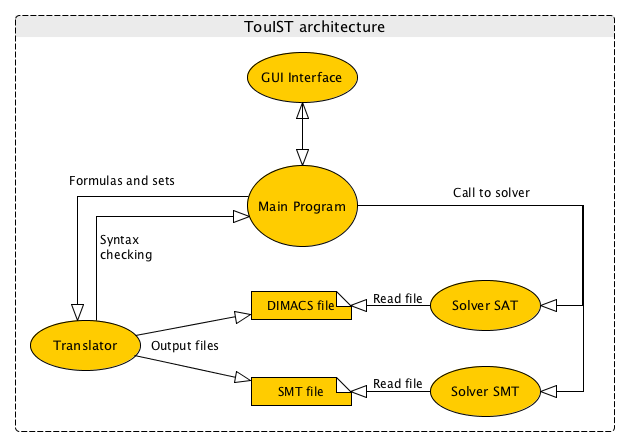
\includegraphics[scale=0.37]{Images/DiagTouist.png}
%   \caption{Architecture de TouIST}
%   \label{fig:architectureTouisT}
% \end{figure}

% Avec \touist on accède à un éditeur puissant et convivial pour éditer des formules logiques complexes et des contraintes variées comme :

% $$\bigwedge_{i \in \{1..9\}} (P_i \IMPL Q_{i+1})$$

% qui abrège confortablement :\\ 

% $(P_1 \IMPL Q_2) \AND (P_2 \IMPL Q_3) \AND \ldots (P_9\IMPL Q_{10})$. 
% \\

% Une fois qu'un ensemble de formules a été donné à l'interface, sa satisfiabilité peut être vérifiée : l'interface peut l'envoyer au prouveur qui retourne un modèle, affiché comme le montre la figure \ref{fig:ExampleOfAModel} si un tel modèle existe. Ensuite par l'intermédiaire de l'interface, l'utilisateur peut par exemple demander d'autres modèles (bouton \guill{Next} de l'interface). Contrairement à \satoulouse qui aurait nécessité de modifier les formules pour interdire le modèle et de relancer le solveur, \touist conserve une instance du solveur en attente, ce qui permet d'obtenir les modèles suivants bien plus rapidement.

% \begin{figure}[htbp]
% \centering
% 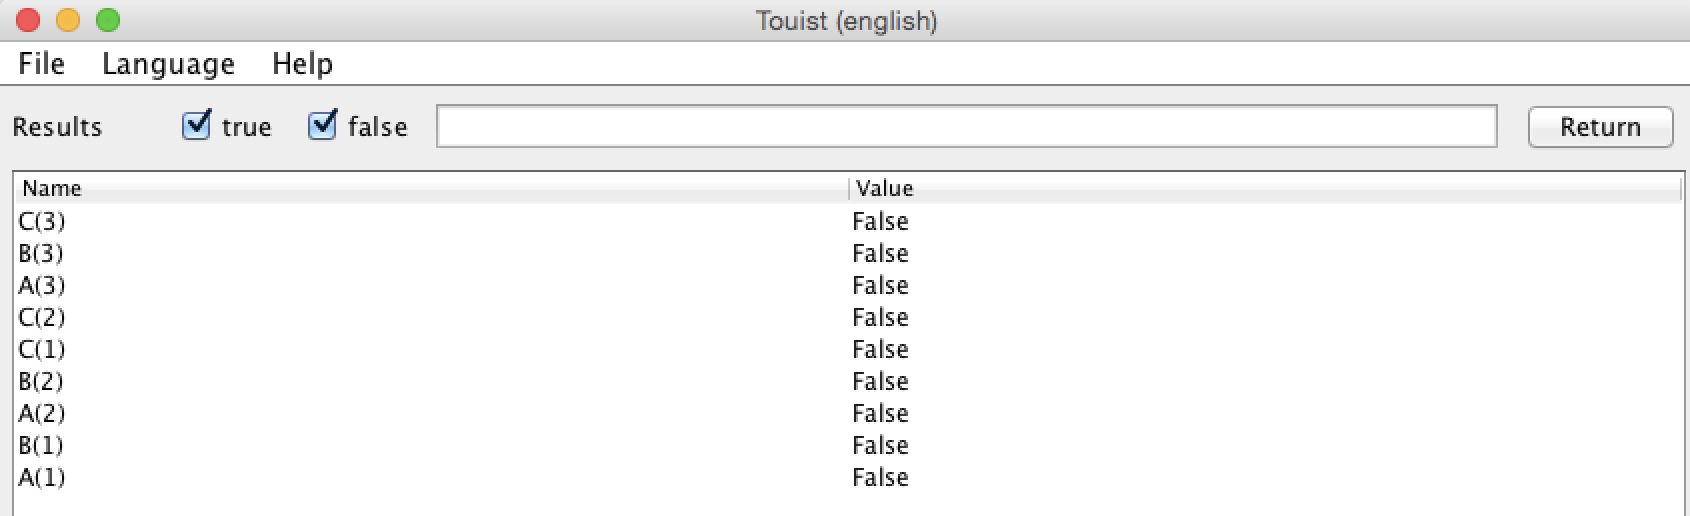
\includegraphics[scale=0.27]{Images/ExampleOfAModel.png}
%   \caption{Affichage de modèle}
%   \label{fig:ExampleOfAModel}
% \end{figure}

% Les modèles renvoyés par le solveur sont totaux : une valeur est affectée \`{a} chacune des variables apparaissant dans les formules envoyées au solveur. L'utilisateur peut sélectionner uniquement les propositions vraies ou les propositions fausses. Il peut également sélectionner des sous-ensembles de variables en tapant une expression régulière pour les filtrer.


% \section{Détail de ce qui peut être fait avec \touist\label{sec:sat_tobedone}}

% \subsection{Ensembles de domaines}
% Avec le temps, nous avons remarqué que nous avions souvent besoin d'écrire des choses comme :
% $$\begin{aligned}\bigwedge_{i \in \{1..9\}} \bigwedge_{j \in \{1..9\}}\bigwedge_{ m\in \{A,B,C,D,E,F,G,H,I\}} \hspace{2cm}\\ \left( P_{i,j,m}\IMPL \bigwedge_{n \in \{A,B,C,D,E,F,G,H,I\}|m\neq n}\NOT P_{i,j,n}\right)\end{aligned}$$
% Si on lit $P_{i,j,m}$ comme  \guill{il y a la lettre $m$ dans la case $(i,j)$} d'une grille $9\times 9$, la formule ci-dessus exprime qu'il y a \emph{au plus} une lettre parmi `A' ... `I' dans chaque case. 

% Ces ensembles $\{1..9\}$ et $\{A,B,C,D,E,F,G,H,I\}$ sont des \emph{ensembles de domaines}, et avec \touist l'utilisateur peut définir autant d'ensembles de domaines qu'il le souhaite, par exemple :

% \begin{verbatim}
%   $N=[1..9]
%   $L=[A,B,C,D,E,F,G,H,I]
% \end{verbatim}

% et ainsi écrire la formule précédente comme :
% $$\bigwedge_{i \in N} \bigwedge_{j \in N}\bigwedge_{ m\in L}P_{i,j,m}\IMPL \bigwedge_{n \in L|m\neq n}\NOT P_{i,j,n}$$
% De plus, les opérations usuelles sur les ensembles ($\cup$, $\cap$, $\setminus$, ...) peuvent être utilisées pour définir d'autres ensembles.


% \subsection{Formules propositionelles}

% Les formules de \touist sont basées sur des variables propositionnelles (qui peuvent être indicées) et les opérateurs logiques usuels ($\AND$, $\OR$, $\IMPL$, $\NOT$, $\IFF$). Ainsi on peut taper des formules usuelles simples comme $Pluie \IMPL Nuages$. Mais en plus, nous fournissons des opérateurs logiques de haut niveau qui permettent d'exprimer des assertions complexes dans une forme très compacte.

% \subsubsection*{Conjonctions et disjonctions généralisées}
% Elles permettent d'exprimer des conjonctions et des disjonctions sur des formules contenant des paramètres qui varient, par exemple :
% \begin{itemize}
% \item $ \bigwedge_{i \in N} P_i$, o\`u $N$ est l'ensemble de domaine défini précédemment.\\
%   Elle représente la conjonction
%   $P_1 \AND P_2 \AND \ldots \AND P_9$. 
% \item $\bigvee_{i \in E} P_i$.
% \end{itemize}

% Bien sûr, ces opérateurs peuvent être imbriqués comme dans :
% $$\bigwedge_{i \in N} \bigwedge_{j \in N}\bigvee_{ m\in L}P_{i,j,m}$$

% qui indique que dans chaque cellule se trouve au moins une lettre.


% \subsubsection*{Contraintes de cardinalité}
% C'était l'un des sujets \guill{laissé pour le futur} de \cite{GaScSt2011}.
% Ces opérateurs logiques moins classiques sont disponibles dans \touist : il permettent de réduire drastiquement la taille de certaines formules, ce sont : $\atM{}{}$, $\atL{}{}$ et $\exact{}{}$.\\ L'exemple suivant décrit leur signification :
% \begin{itemize}
% \item $\atM{i \in N}{2} P_i$ représente \guill{pour au plus deux valeurs de $i \in N$ $P(i)$ est vraie};
% \item $\atL{i \in N}{2} P_i$ représente \guill{pour au moins deux valeurs de $i \in N$ $P(i)$ est vraie};
% \item $\exact{i \in N}{2} P_i$ représente \guill{pour exactement deux valeurs de $i \in N$ $P(i)$ est vraie}.
% \end{itemize}
% La disjonction généralisée est en fait un cas particulier de ceci (au moins une est vraie), la conjonction aussi (au plus 0 est fausse), et le ou exclusif peut être vu comme exactement une parmi deux est vraie. \\
% Rappelons qu'avec des opérateurs logiques classiques et avec $N$ contenant 9 éléments, $\atM{i \in N}{3} P_i$ devrait nécessiter une formule contenant 84 propositions $P_i$ puisque cela revient à choisir 3 parmi 9 ce qui donne $\binom{9}{3}$ possibilités, et ni $\bigwedge$ ni $\bigvee$ n'aideraient beaucoup. 

% \subsubsection*{Contraintes et calculs sur des indices}

% Souvent nous avons besoin d'ajouter des contraintes sur les indices, par exemple :
% $$\bigwedge_{i \in E } \bigwedge_{j \in E  | i \neq j}P_{i,j}$$
% qui signifie que $P_{i,j}$ est vraie lorsque $i\neq j$. 

% C'était la seule contrainte disponible dans \satoulouse, maintenant dans \touist la gamme de possibilités à été largement enrichie. Les contraintes peuvent inclure des opérateurs usuels de comparaison comme $<$, $>$, $\leq$, $\geq$, $\neq$, $=$ et ces comparaisons peuvent s'appliquer non seulement aux indices, mais aussi à toute expression arithmétique impliquant des indices et $+$, $-$, $*$, $/$, $\mod$, $\sqrt{\phantom{x}}$. 

% Exprimer une phrase comme \guill{chaque case $(i,j)$ contient un nombre qui n'est pas égal à $i+j$} donnera :
% $$\bigwedge_{i \in N } \bigwedge_{j \in N} \bigvee_{k \in N|k\neq i+j} P_{i,j,k}$$
% Bien sûr, \emph{toutes ces phrases} pourraient être exprimées avec les opérateurs logiques usuels bruts, mais ceci serait un travail fastidieux. Néanmoins, les étudiants doivent savoir ce qui est derrière la scène, et qu'une telle formule est l'abréviation de quelque chose comme :
% $$P_{1,1,1}\vee P_{1,1,3}\vee P_{1,1,4}\ldots P_{1,2,1}\vee P_{1,2,2}\vee P_{1,2,4}\vee \ldots $$
% qui est très long et terne.



% \subsection{Aspects techniques}

% \subsubsection*{Langage d'entrée vs Langage d'affichage}

% Les formules que nous avons vues précédemment sont écrites dans le \emph{langage d'affichage} (style \LaTeX), mais tous ces symboles ne sont pas disponibles sur les claviers, ainsi pour écrire les formules et ensembles de domaines, l'utilisateur utilisera le \emph{langage d'entrée}.
% Par exemple, la formule précédente avec l'ensemble associé $N$ sera tapée (les variables sont préfixées par \$) :
% \begin{verbatim}
% bigand $i,$j in $N,$N:
%   bigor $k in $N when $k != $i+$j:
%     P($i,$j,$k)
%   end
% end
% \end{verbatim}
% Mais \touist les affiche immédiatement en style \LaTeX\ comme on peut le voir dans le panneau droit montré sur la figure \ref{fig:LatexDisplay}.
% La définition de l'ensemble $N$ est faite dans l'onglet \guill{Ensembles}.

% \begin{figure*}[htbp]
% \centering
% 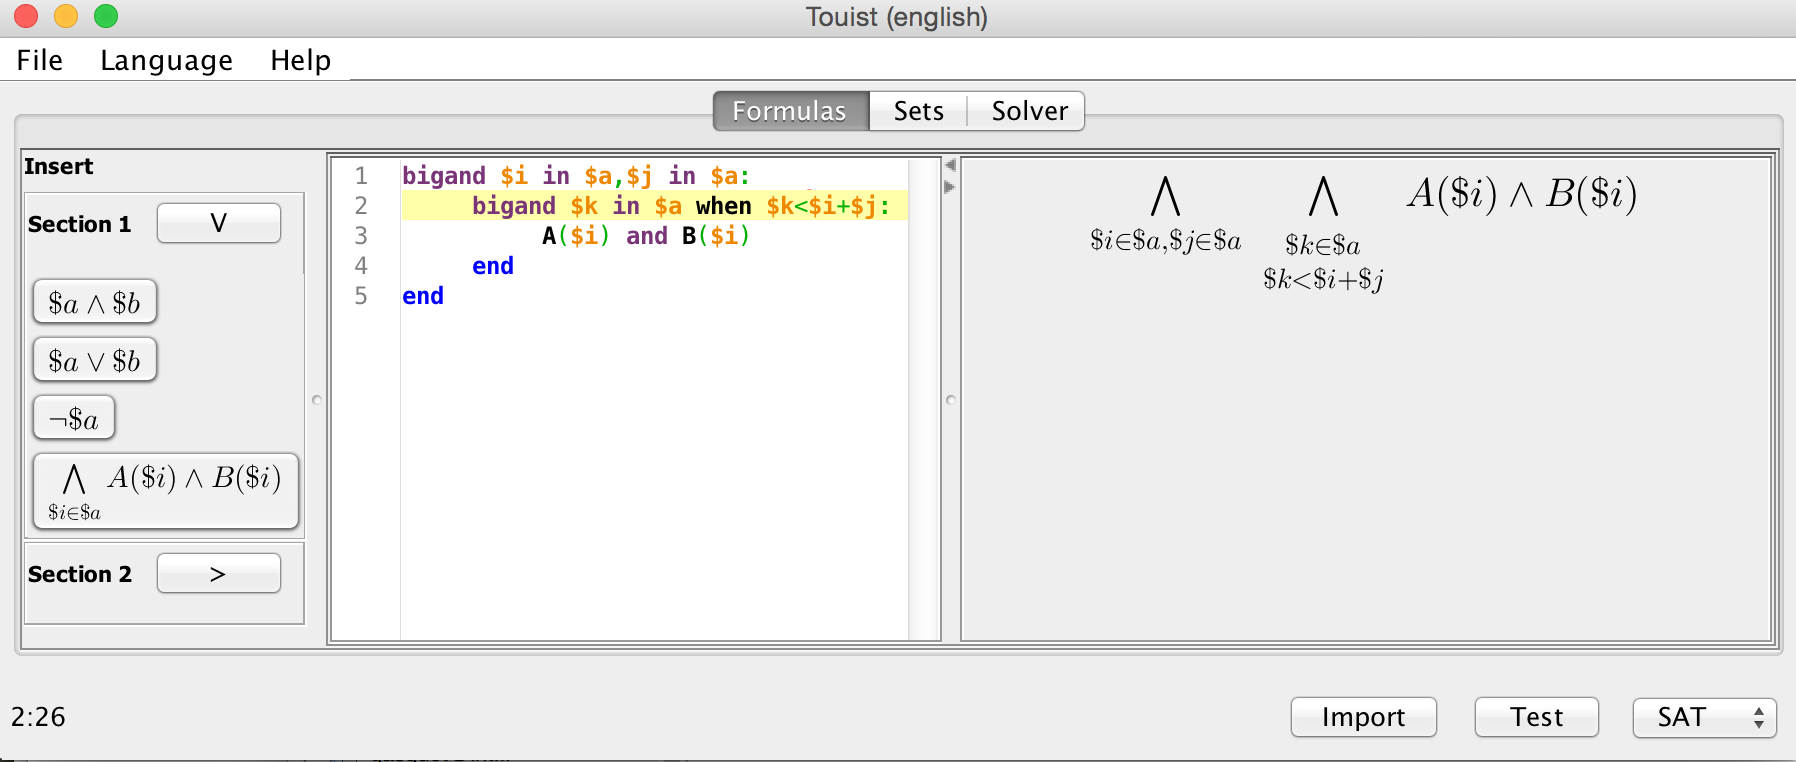
\includegraphics[scale=0.45]{Images/LatexDisplay.png}
%   \caption{Affichage en style \LaTeX}
%   \label{fig:LatexDisplay}
% \end{figure*}


% En outre, les formules peuvent être tapées à la main dans la fenêtre d'édition, ou introduites dans une sorte d'éditeur dirigé par la syntaxe, en raffinant progressivement l'arbre syntaxique, ou encore elles peuvent être importées à partir d'un fichier externe.





%\begin{figure*}[ht]
%  \centering
%  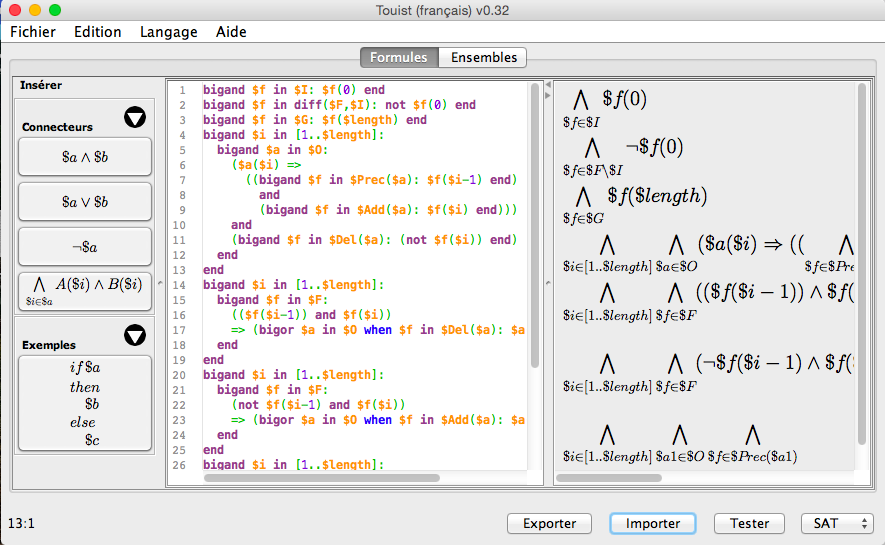
\includegraphics[scale=.4]{touist1.png}
%  \caption{Interface de TouIST}
%  \label{fig:touist}
%\end{figure*}


%%......................................................................
%\section{Behind the scenes}\label{sec:sat_behind}
%
%% !TeX root = IAF2015-TouIST.tex
% la ligne précédente sert pour le logiciel TexWorks afin de pouvoir compiler ce fichier directement sans devoir ouvrir satoulouse_main.tex!
The piece of software \satoulouse is an open-source project globally written in
JAVA so that it can be used on many different platforms.

\subsection{The graphical user interface}


The graphical user interface (GUI) enables the user to write formulas and to
click on the button ``check if the set of formulas is satisfiable''. The GUI
is written in JAVA in order to be able to use the suitable library SWING. In
particular, as this library is object oriented, it was really simple to create
our own widget to enter a formula of propositional logic. Formulas are also
displayed in \LaTeX\ style thanks to the library jLatexMath\footnote{\url{http://forge.scilab.org/index.php/p/jlatexmath/}} which does not require any
additional software (in particular it does not require a real \LaTeX\
installation).


\subsection{The SAT solver}

The SAT solver used as backend of \satoulouse\ is SAT4J
\footnote{\url{http://www.sat4j.org/}}. The first advantage of this solver is
that it is written in JAVA so it is easy to call it from the GUI. The second
one is its good efficiency \cite{berre10:_sat4j}, and even if it is not the best SAT
solver in the world (see SAT Race 2008), it is one of the best. 


\subsection{Connection between the SAT solver and the graphical user interface}

The translation from formulas written by the user to formulas for the SAT
solver SAT4J is divided in two parts:
\begin{itemize}
\item expanding formulas, that is to say, rewrite macros into expanded
  conjunction normal forms. For instance, we expand the formula $\bigwedge_{i
    \in \{1 .. 4\}} p_i$ into $(((p_1 \land p_2) \land p_3) \land
  p_4)$. Expanding formulas is done in Scheme code intepreted with the JAVA
  library kawa \cite{bothner1998kawa}. Scheme is a suitable language to
  perform this translation because parsing of formulas is directly done in
  this language: formulas are directly s-expressions.

\item translating the expanded conjunctive normal forms into a rigorous SAT4J
  input. This part is done in Java because we need to run SAT4J which is coded
  in JAVA. We construct a map between the propositions of the GUI (strings)
  and strict positive integers used by SAT4J and then build corresponding
  arrays of integer for SAT4J.
\end{itemize}



\subsection{Loading and saving a problem}

As we can give explicit names to propositions (and not only integers as for
SAT4J), as we have macros (like $\bigwedge_{i \in \{1 .. 4\}} switch_i$),
\satoulouse\ has its own file format: we simply write s-expressions representing
formulas. Nevertheless, \satoulouse\ is also able to load standard DIMACS cnf
format files as depicted below.\\[0pt]


%\begin{figure}
%\begin{center}
\begin{minipage}{6cm}
\begin{center}
\begin{verbatim}
c A sample .cnf file. 
p cnf 3 2
1 -3 0
2 3 -1 0 
1 2 -3 0
\end{verbatim}
\end{center}
\end{minipage}
\begin{minipage}{6cm}
\mbox{  }\\[18pt]
$((p_1 \vee \neg p_3) \wedge$

$(p_2 \vee p_3 \vee \neg p_1) \wedge$

$ (p_1 \vee p_2 \vee \neg p_3))$s
\end{minipage}
%\end{center}
%\caption{
\begin{center}The standard DIMACS cnf format\label{figure:dimacsformat}\end{center}
%}
%\end{figure}

%\begin{figure}
%%\begin{center}
%\begin{tabular}{lll}
%%\begin{center}
%%\begin{verbatim}
% c A sample .cnf file. & &\\
%p cnf 3 2 & \\
%1 -3 0  & \phantom{xxxxxxxxxxxxxxx} & $((p_1 \vee \neg p_3) \wedge$ \\
%2 3 -1 0  & & $(p_2 \vee p_3 \vee \neg p_1) \wedge$\\
%1 2 -3 0 & & $ (p_1 \vee p_2 \vee \neg p_3))$
%%\end{verbatim}
%%\end{center}
%\end{tabular}
%\caption{The standard DIMACS cnf format\label{figure:dimacsformat}}
%\end{figure}

%%% Local Variables: 
%%% mode: latex
%%% TeX-master: "satoulouse_main"
%%% End: 

%

% %......................................................................
% \section{Sujets avancés pour les étudiants de cycles supérieurs}\label{sec:advanced_topics}
% %......................................................................


% Dans ce qui suit, nous présentons très succictement quelques fonctionnalités avancées de \touist. Elles devraient intéresser les étudiants de cycles supérieurs et leurs enseignants bien sûr. Elles concernent SMT (SAT Modulo Theories), la planification par satisfaction de base de clauses (planification SAT) et leur combinaison la planification SMT.


% \subsection{SMT: SAT Modulo Theories}

% Certains problèmes combinatoires nécessitent néanmoins de traiter des calculs sur les nombre naturels ou réels. Ceci peut être fait en utilisant seulement la logique propositionnelle (par exemple, $2+3=5$ pourrait être codé par $add_{2,3,5}$), mais c'est très inconfortable à moins qu'il n'y ait que quelques additions à faire. Ne parlons même pas des opérations de multiplication ou plus complexes. L'idée derrière la genèse de SMT a été de combiner des solveurs SAT avec un solveur arithmétique dans le but d'améliorer le traitement de la partie arithmétique du raisonnement. Dans de nombreux cas, ceci n'améliorera pas seulement l'efficacité du solveur, mais permettra aussi d'exprimer les contraintes arithmétiques des problèmes d'une manière radicalement plus compacte.

% Pensez au jeu de Kamaji\footnote{\url{http://fr.wikipedia.org/wiki/Kamaji}}  o\`u le joueur doit grouper des nombres adjacents dans une grille de sorte que leur somme soit égale à un nombre fixe. Résoudre le jeu nécessite essentiellement un raisonnement logique mais a aussi besoin d'un peu d'arithmétique (addition).


% Si $x_{i,j}$ pour chaque case $(i,j)$ est un entier et $G(i,j,i,k)$ représente le fait que les cases $(i,j)$ à $(i,k)$ de la ligne $i$ forment un groupe, la contrainte de somme pourrait être exprimée par :
% $$\sum_{m\in E}x_{i,m}=N$$
% o\`u $N$ est le nombre fixe et $E$ est $\{j,j+1,\ldots,k\}$. La logique propositionnelle pure n'est certainement pas adaptée pour de telles phrases !




% \subsection{\touist pour la planification classique SAT}

% En Intelligence Artificielle, la \emph{planification} est un processus cognitif qui consiste à générer automatiquement, au travers d'une procédure formelle, un résultat articulé sous la forme d'un système de décision intégré appelé \emph{plan}. Le plan est généralement sous la forme d'une collection organisée d'\emph{actions} et il doit permettre à l'univers d'évoluer de l'\emph{état initial} à un état qui satisfait le \emph{but}. Dans le cadre classique, le plus restrictif, on considère les actions comme des transitions instantanées sans prendre en compte le temps.

% La planification par satisfaction de base de clauses (planification SAT) a été introduite avec le planificateur SATPLAN \cite{kautzS92_planning_sat}. Dans cette approche, on travaille directement sur un ensemble fini de variables propositionnelles. Deux actions identiques pouvant apparaître à des endroits différents d'un même plan doivent pouvoir être différenciées et on leur associe donc des propositions différentes. Comme on ne connaît pas à l'avance la longueur d'un plan solution d'un problème, on ne peut pas créer un codage unique permettant de le résoudre puisqu'il faudrait créer une infinité de variables propositionnelles pour représenter toutes les actions de tous les plans possibles. La solution la plus commune consiste alors à créer un codage représentant tous les plans d'une longueur $k$ fixée. La base de clause ainsi obtenue est donnée en entrée à un solveur SAT qui retourne, lorsqu'il existe, un modèle de cette base. Le décodage de ce modèle permet alors d'obtenir un plan-solution. Si la résolution du codage ne donne pas de modèle, la valeur de $k$ est augmentée et le processus réitéré. Pour la complétude du procédé, tous ces modèles doivent correspondre exactement à tous les plans solutions d'une longueur fixée du problème.


% Une différence importante de \touist, en comparaison avec \satoulouse, est sa capacité à prendre en compte à la fois des formules logiques et ensembles de domaines. Par exemple, si l'on veut résoudre un problème de planification particulier, \satoulouse est facile à utiliser pour décrire le problème et le résoudre via un solveur SAT. Mais si notre objectif est de résoudre plusieurs problèmes de planification génériques, nous pouvons profiter de la flexibilité de \touist qui permet à l'utilisateur de décrire une méthode générique de résolution avec des règles encodées comme formules et d'utiliser des ensembles de domaines pour décrire chaque problème de planification particulier. De nombreuses règles de codage pour la résolution de problèmes de planification ont déjà été proposées \cite{kautzS92_planning_sat,MaliK99_plan_space_encodings,Rintanen:2006}. Comme exemple d'une telle règle nous donnons ci-après un codage des \emph{frame-axioms}. Si un fait est faux à une étape $i-1$ d'un plan solution et devient vrai à l'étape $i$, alors la disjonction des actions qui peuvent établir le fait à l'étape $i$ du plan est vraie. C'est à dire, au moins une action qui établit le fait doit avoir été appliquée.


%   \[\begin{aligned}\bigwedge_{i\in\{1..longueur\_plan\}}
%   \bigwedge_{f\in Faits} \hspace{4cm}\\
%   \left((\lnot f(i-1) \wedge f(i)) \Rightarrow 
%   \bigvee_{a\in Actions / f\in Effets(a)} a(i)\right)\end{aligned}\]
% \\


% \subsection{\touist pour la planification temporelle SMT}

% Pour résoudre des problèmes de planification réels, l'une des principales difficultés à surmonter consiste à prendre en compte la dimension temporelle. En effet, de nombreux problèmes du monde réel nécessitent, pour être résolus ou exécutés plus efficacement, la prise en compte de la durée des actions, des instants auxquels des évènements se produisent, ou encore la concurrence d'actions.

% En complément de SAT, notre nouvelle plateforme \touist est capable de gérer des théories comme la différence logique ou l'arithmétique linéaire sur les nombres entiers (QF\_IDL, QF\_LIA) ou les nombres réels (QF\_RDL, QF\_LRA), et d'appeler un solveur SMT pour trouver une solution. Pour être résolus, les problèmes de planification temporelle issus du monde réel nécessitent une représentation continue du temps, et donc, l'utilisation de nombres réels dans les codages logiques. \touist peut être utilisé pour résoudre de tels problèmes impliquant des actions avec durée, des évènements exogènes et des buts temporellement étendus, par exemple avec les règles de codage proposées dans \cite{MarisRegnier08}. Nous donnons ci-après un codage des exclusions mutuelles temporelles d'actions. Si deux actions $a$ et $b$ produisant respectivement une proposition $p$ et sa négation sont actives dans le plan ($a \wedge b$ est vrai), alors l'intervalle de temps $[\tau(a \mid\rightarrow p), \tau(a \rightarrow\mid p)]$ correspondant à l'activation de $p$, et l'intervalle de temps $[\tau(b \mid\rightarrow \lnot p), \tau(b \rightarrow\mid \lnot p)]$ correspondant à l'activation de $\NOT p$ sont disjoints. Dans ce cas, il faut ajouter une disjonction pour imposer que la fin de l'un de ces intervalles soit strictement avant le début de l'autre.

%   \[\bigwedge_{a\in Actions}
%   \bigwedge_{b\in Actions}
%   \bigwedge_{f\in Faits | f\in Effets(a) \wedge \lnot f\in Effets(b)}\]
%   \[\left(\left(a \wedge b\right) \Rightarrow 
%   \left( \begin{aligned} \left(\tau(b \rightarrow\mid \lnot f) < \tau(a \mid\rightarrow f)\right)
%     \\ \vee
%     \left(\tau(a \rightarrow\mid f) < \tau(b \mid\rightarrow \lnot f)\right)
%  \end{aligned} \right)\right) \]


%----------------------------------------------------------------------

%\vspace{-1cm}

%%%%%%%%%%%%%%%%%%%%%%%%%%%%%%%%%%%%%%%%%%%%%%%%%%%%
%%%%%%%%%%%%%%%%%%%%%%%%%%%%%%%%%%%%%%%%%%%%%%%%%%%%
\section{Description du \game}
%%%%%%%%%%%%%%%%%%%%%%%%%%%%%%%%%%%%%%%%%%%%%%%%%%%%
%%%%%%%%%%%%%%%%%%%%%%%%%%%%%%%%%%%%%%%%%%%%%%%%%%%%
\label{sec:gameDescription}
Le principe du \game est le suivant : on dispose au départ d'un nombre $\nbAllumettes$ non nul d'allumettes
% IL EST IMPORTANT DE SPECIFIER QUE LE NB D'ALLUMETTES EST NON NUL CAR NOTRE DEF DE 0_PERD NE DEFINIT CETTE NOTION QUE POUR t>0 !!!
et un nombre $\nbJoueurs$ de joueurs peuvent prendre $1$ ou plusieurs allumette(s). Le joueur qui perd est celui qui, le premier, ne peut plus prendre d'allumette.\footnote{Il existe différentes variantes de ce jeu, notamment en faisant varier les nombres d'allumettes et de joueurs, mais également en faisant varier les actions possibles ou en introduisant des contraintes (par exemple, on ne peut pas prendre le même nombre d'allumettes que le joueur précédent).} Le nombre de tours de jeu possibles est au plus égal à celui des allumettes (à minima, chaque joueur ne prend à chaque tour qu'une seule allumette). Ainsi, l'ensemble des indices des tours possibles est $\turnsSet = \{ 0, ..., \nbAllumettes \}$ où $0$ est l'indice de l'état initial. De même, l'ensemble des nombres possibles d'allumettes encore disponibles est $\matchesSet = \{ 0, 1, ..., \nbAllumettes \}$.

Afin de simplifier au maximum le langage utilisé, nous modélisons ici une variante où $\nbAllumettes = 4$ et $\nbJoueurs = 2$. Les joueurs sont notés $0$ et $1$ et c'est au tour de $0$ de jouer au tour $t$ ssi $\turn{t}$ est vrai (considérant que si ce n'est pas le tour de $0$ alors c'est celui de $1$). De plus, $\rest{t}{n}$ est vrai ssi au tour $t$ il reste $n$ allumettes.

Ainsi, l'état initial du jeu est le suivant : 
\begin{gather}
\rest{0}{\nbAllumettes} \land \turn{0}
\label{eq:initialState}
\end{gather}
indiquant qu'au tour $0$ il y a encore $\nbAllumettes$ de disponible et que c'est au tour de $0$ de jouer.

Dans la version présentée ici du \game, on limite également le nombre des actions possibles à deux : un joueur peut prendre soit $1$ allumette, soit $2$ allumettes. Ainsi, $\takes{t}$ est vrai ssi un agent prend $2$ allumettes au tour $t$ (considérant ainsi que $\takes{t}$ est faux ssi il n'en prend qu'une). 

Ainsi :
\begin{align}
\begin{split}
\bigwedge_{\substack{t \in \turnsSet\\ n \in \matchesSet\\ n \geq 2}}
    \bigg ( & \Big ( \rest{t}{n} \land \takes{t} \limp\\
    & \hspace{1.5cm}\rest{t+1}{n-2} \ \Big ) \; \land \\
    & \Big ( \rest{t}{n} \land \neg \takes{t} \limp \\
    & \hspace{1.5cm}\rest{t+1}{n-1} \Big ) \bigg )
\end{split}
\end{align}
capture le fait que si au tour $t$ il reste au moins $2$ allumettes et qu'un joueur en prend $2$ alors au tour suivant il en reste $2$ de moins, et que si il n'en prend qu'une alors au tour suivant il en reste $1$ de moins.

En revanche, si au tour $t$ il reste exactement $1$ allumette, alors nécessairement le joueur en prendra $1$ et il en restera $0$ au tour suivant :
\begin{gather}
\bigwedge_{t \in \turnsSet}
    \Big (\rest{t}{1} \limp \neg \takes{t} \land \rest{t+1}{0}\Big )
\end{gather}

Notre modèle spécifie ensuite que :
\begin{align}
& \bigwedge_{t \in \turnsSet}
    \bigvee_{n \in \matchesSet}
        \rest{t}{n} \\
& \bigwedge_{\substack{t \in \turnsSet\\ n1, n2 \in \matchesSet\\ n1 \neq n2}}
    \Big ( \rest{t}{n1} \limp \neg\rest{t}{n2} \Big )
\end{align}
La première formule stipule qu'à chaque tour $t$ il existe au moins un nombre $n$ d'allumettes restant, et la seconde que ce nombre est unique.

\begin{figure*}
\centering
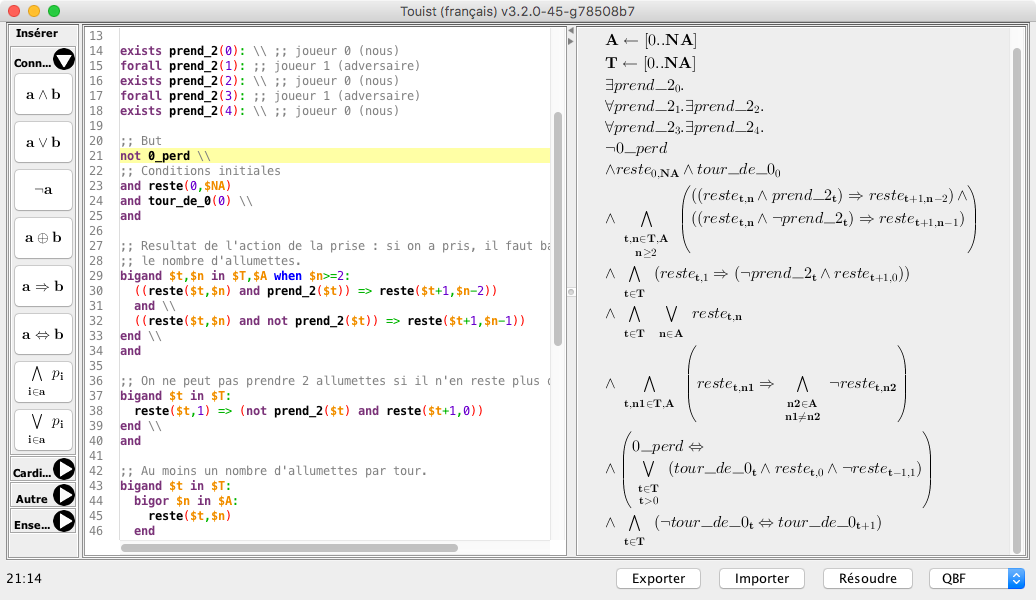
\includegraphics[width=0.9\textwidth]{Pictures/touistScreenshot}
\caption{Capture d'écran de \touist avec le \game. Le fichier est disponible à l'adresse \url{https://github.com/maelvalais/allumettes}}
\label{fig:touistScreenshot}
\end{figure*}

Il faut maintenant définir quand un joueur a perdu :
\begin{gather}
\begin{split}
\lost \lequiv \bigvee_{\substack{t \in \turnsSet\\ t > 0}} & \bigg ( \turn{t} \land \rest{t}{0} %\land \\
%    &  \Big ( \rest{t-1}{1} \lor \rest{t-1}{2} \Big 
\bigg )
\end{split}
\end{gather}
signifie que le jouer $0$ a perdu ssi il existe un tour $t$ où il reste $0$ allumettes alors qu'à l'instant d'avant il y en avait au moins une.

Finalement, à chaque tour $t$, ce n'est pas au joueur $0$ de jouer ssi c'est à lui de jouer au tour suivant :
\begin{gather}
\bigwedge_{t \in \turnsSet \setminus \{ \nbAllumettes \} } \Big (
    \neg \turn{t} \lequiv \turn{t+1}
\Big )
\label{eq:turnChange}
\end{gather}



%%%%%%%%%%%%%%%%%%%%%%%%%%%%%%%%%%%%%%%%%%%%%%%%%%%%
%%%%%%%%%%%%%%%%%%%%%%%%%%%%%%%%%%%%%%%%%%%%%%%%%%%%
\section{Formalisation d'une stratégie gagnante à l'aide de QBF}
%%%%%%%%%%%%%%%%%%%%%%%%%%%%%%%%%%%%%%%%%%%%%%%%%%%%
%%%%%%%%%%%%%%%%%%%%%%%%%%%%%%%%%%%%%%%%%%%%%%%%%%%%
\label{sec:QBFandTouist}
Dans cette section, nous allons présenter à l'aide de notre exemple du \game l'extension de \touist à Quantified Boolean Formulas (QBF) connu comme étant le problème de référence pour la classe de complexité PSPACE (\cite{Stockmeyer:1973:WPR:800125.804029}). C'est une extension de la logique propositionnelle permettant de quantifier sur les variables propositionnelles. 

Par exemple, $\forall p \exists q.p \leftrightarrow q$ se lit : pour toute valeur de vérité de $p$, il existe une valeur de vérité de $q$ tel que $p \leftrightarrow q$ est vrai. Cette formule est vraie (il suffit de choisir la même valeur pour $q$ que pour $p$). Alors que  $\exists p \forall q.p \lor q$ ne l'est pas. Ainsi, une formule booléenne quantifiée est toujours SOIT vraie SOIT fausse. 

De fait, à toute formule QBF peut être associée une formule propositionnelle sans variables car par définition : 
$\forall p.\Phi$ est vraie ssi $\Phi_{[p:=\top]} \wedge \Phi_{[p:=\bot]}$ l'est, et $\exists p.\Phi$ est vraie ssi $\Phi_{[p:=\top]} \vee \Phi_{[p:=\bot]}$. 

La formule QBF peut être exponentiellement plus compacte que la formule propositionnelle correspondante. 

Par exemple à la formule $\forall p \exists q.p \leftrightarrow q$ correspond la formule propositionnelle \\
$\Big ( (\top \leftrightarrow \top)\vee (\top \leftrightarrow \bot) \Big ) \wedge \Big ( (\bot \leftrightarrow \top)\vee (\bot \leftrightarrow \bot) \Big )$

Le langage de QBF permet d'exprimer naturellement et de manière concise l'existence de stratégies gagnantes ainsi que décrit dans \cite{DBLP:series/txtcs/KroeningS16}. Les coups du joueur 0 (pour lequel on cherche une stratégie gagnante) seront existentiellement quantifiés alors que ceux de son adversaire seront universellement quantifiés. (On cherche les coups du joueur $0$ qui le mèneront à la victoire quels que soient les coups joués par le joueur $1$.)

\touist a été étendu pour être compatible avec le solveur QBF \emph{Quantor 3.2} \cite{Biere:2004:RE:2103144.2103150}. La sélection de ce prouveur dans \touist autorise \emph{de facto} l'utilisation des quantificateurs $\forall$ et $\exists$ (respectivement définis par \verb+exists+ et \verb+forall+ dans \touist).

\begin{figure}
\centering
\tikzset{%
    prend1/.style={->,dotted,very thick,>=latex},
    prend2/.style={->,very thick,>=latex}%
}

\begin{tikzpicture}
% définition des noeuds
\node (t0) at (0.5,0) {4};
\node (t11) at (-1,-1) {2};
\node (t12) at (2,-1) {3};
\node (t21) at (-2,-2) {0};
\node (t22) at (0,-2) {1};
\node (t23) at (1,-2) {1};
\node (t24) at (3,-2) {2};
\node (t31) at (0,-3) {0};
\node (t32) at (1,-3) {0};
\node (t33) at (2,-3) {0};
\node (t34) at (4,-3) {1};
\node (t4) at (4,-4) {0};
% 0 joue
\draw[prend2] (t0)--(t11);
\draw[color=red][prend1] (t0)--(t12);
% 1 joue
\draw[prend2] (t11)--(t21);
\draw[prend1] (t11)--(t22);
\draw[color=red][prend2] (t12)--(t23);
\draw[color=red][prend1] (t12)--(t24);
% 0 joue
\draw[prend1] (t22)--(t31);
\draw[color=red][prend1] (t23)--(t32);
\draw[color=red][prend2] (t24)--(t33);
\draw[prend1] (t24)--(t34);
% 1 joue
\draw[prend1] (t34)--(t4);
\end{tikzpicture}

\caption{Solutions pour le \game (4 all./2 joueurs), en rouge : stratégie gagnante du joueur 0}
\label{fig:solutions}
\vspace{-0.5cm}\end{figure}

\tikzset{%
    prend1/.style={->,dotted,very thick,>=latex},
    prend2/.style={->,very thick,>=latex}%
}


\figurename~\ref{fig:solutions} présente l'ensemble exhaustif des solutions de notre exemple. La racine de l'arbre représente le nombre initial d'allumettes, et chaque flèche l'action de retirer $1$ (\tikz{\draw[prend1] (0,0) -- (1,0)}) ou $2$ (\tikz{\draw[prend2] (0,0) -- (1,0)}) allumette(s). Au bout de la flèche, le nombre d'allumettes après exécution de l'action concernée. D'après cette figure, on voit que si le joueur $0$ commence (ce qui est imposé par (\ref{eq:initialState})) et qu'il retire une seule allumette (il en reste donc 3) on voit qu'il a une stratégie gagnante : 
\begin{itemize}
\item si le joueur $1$ retire ensuite $2$ allumettes il en restera $1$ seule que le joueur $0$ peut retirer pour gagner (puisque le joueur $1$ ne pourra ensuite plus retirer d'allumette) ;

\item si le joueur $1$ retire une seule allumette, il en restera  $2$ et le joueur $0$ pourra au coup suivant les retirer en un seul coup et le joueur $1$ perd.
\end{itemize}

Nous tirons parti de QBF pour écrire cette stratégie dans \touist. Si on note $\Phi$ la conjonction des formules (\ref{eq:initialState}) à (\ref{eq:turnChange}) alors la recherche d'une stratégie gagnante pour le joueur $0$ s'écrit simplement :
\vspace{-0.2cm}
\begin{align}
\begin{split}
&\exists \takes{0}
\forall \takes{1}\\
&\qquad\exists \takes{2}
\forall \takes{3} \\
&\quad\exists \takes{4}\text{ . }\neg \lost \land \Phi
\end{split}
\end{align}

\noindent
Autrement dit, on cherche à satisfaire le fait qu'il existe une action du joueur $0$ au tour $0$ telle que quelle que soit l'action du joueur $1$ au tour $1$, il existe une action du joueur $0$ au tour $2$, telle que pour toute action du joueur $1$ au tour $3$ il existe une action du joueur $0$ (qui sera donc le dernier à jouer) telle que le joueur $0$ ne perd pas et que les contraintes inhérentes au \game soient satisfaites.

% \warning{[DOMI : ] Je ne suis pas sûr de ce qui suit car je n'arrive pas à faire fonctionner le prog des allumettes avec la dernière version de \touist (ça plante).}

L'exécution du programme dans \touist indique que cette formule est vraie, ce qui signifie l'existence d'une stratégie gagnante pour le joueur $0$. Le solveur retourne la valeur des (ici une seule) variables existentielles correspondant au prochain coup du joueur $0$. À ce stade, le joueur adverse doit fournir son coup qui fixe la valeur des variables universelles correspondant à ses possibles prochains coups. On exécute alors de nouveau le programme modifié de la façon suivante (de manière à prendre en compte le calcul de la valuation de $\takes{0}$) :
\begin{align*}
\begin{split}
&\exists \takes{0}
\exists \takes{1}\\
&\qquad\exists \takes{2}
\forall \takes{3} \\
&\quad\exists \takes{4}\text{ . }\neg \lost \land c_0 \land c_1 \land  \Phi
\end{split}
\end{align*}
où $c_0$ est soit $\takes{0}$ soit $\neg \takes{0}$ en fonction du coup du joueur $0$, et similairement pour $c_1$ en fonction du coup choisi par l'adversaire. La  situation après ces deux coups est la nouvelle situation initiale pour le solveur et la recherche du coup suivant du joueur $0$... jusqu'à sa victoire ! On réitère ce processus jusqu'à ce que toutes les variables aient reçu une valeur. 
%On obtient alors :
%\begin{gather*}
%\interpret[\takes{0}] = 0, 
%\interpret[\takes{1}] = 1 
%\interpret[\takes{2}] = 0
%\end{gather*}
%qui se lit : pour que le joueur $0$ gagne il doit prendre $1$ allumette, le joueur $1$ en prend $2$, puis le joueur $0$ en prend $1$.

%%%%%%%%%%%%%%%%%%%%%%%%%%%%%%%%%%%%%%%%%%%%%%%%%%%%
%%%%%%%%%%%%%%%%%%%%%%%%%%%%%%%%%%%%%%%%%%%%%%%%%%%%
\section{Conclusion}
%%%%%%%%%%%%%%%%%%%%%%%%%%%%%%%%%%%%%%%%%%%%%%%%%%%%
%%%%%%%%%%%%%%%%%%%%%%%%%%%%%%%%%%%%%%%%%%%%%%%%%%%%

\touist peut être vu comme un compilateur de langages logiques étendus et de haut niveau vers des prouveurs efficaces indépendants. Ces deux facettes lui confèrent une grande facilité d'utilisation, un large spectre d'application et de bonnes performances calculatoires. À ce titre, il constitue un outil complètement original et unique en son genre. 

Nous l'utilisons dans le cadre du cours d'initiation à la logique en % va t'en
licence d'informatique, mais aussi en master, dans le cadre de travaux pratiques et de projets. Les étudiants sont ainsi appelés à parcourir tout le processus allant de la formalisation à la résolution de problèmes qui vont au-delà des problèmes-jouets faisables sur papier. 

Mais plus encore, \touist\ est d'ores et déjà  utilisé par des chercheurs dans le cadre de travaux mené au sein de notre laboratoire et impliquant une modélisation logique (planification, raisonnement épistémique via traduction en QBF,\ldots), il comble un manque existant au sein des logiciels de calculs formels comme Maple, SageMath, Mathematica ou Maxima qui n'intègrent qu'anecdotiquement des outils logiques.


\appendix
%\section{Code \touist du problème}


% Bibliographie en utilisant BibTeX
\bibliography{biblio}


\end{document}


